%
% Reproducibility manuscript: describe results from relative
% alchemical free energy simulation done with various MD packages.
%
% arara: make
% arara: pdflatex
% arara: bibtex
% arara: pdflatex
% arara: pdflatex
% arara: clean: {files: [reprod.aux, reprod.bbl, reprod.blg, reprod.log, 
%acs-reprod.bib, reprod.lod, reprod.fls]}
%

\documentclass[journal=jctcce,manuscript=article]{achemso}

\usepackage[T1]{fontenc}
\usepackage{graphicx}
\usepackage{amsmath,amssymb,mathrsfs}
\usepackage{xr}
\usepackage{booktabs}
\usepackage{multirow}
\usepackage{rotating}
\usepackage{siunitx}
\usepackage{nameref}
\usepackage{easy-todo}
\usepackage{footref}


\externaldocument[S-]{SI}

\sisetup{
  separate-uncertainty = true
}

\newcommand{\progname}[1]{\texttt{#1}}
\newcommand{\inpopt}[1]{\texttt{#1}}

\renewcommand{\vec}[1]{\mathbf{#1}}
\renewcommand{\footnoterule}{}


\title{Are Alchemical Free Energy Calculations Reproducible? (draft)}


\author{Hannes H. Loeffler}
\affiliation[Scientific Computing Department, STFC]{Science \&
  Technology Facilities Council, Daresbury, Warrington, WA4 4AD,
  United Kingdom}
\email{Hannes.Loeffler@stfc.ac.uk} \phone{+44 1925 603367}

\author{Stefano Bosisio}
\affiliation[University of Edinburgh]{EaStCHEM School of Chemistry,
  University of Edinburgh, David Brewster Road, Edinburgh EH9 3FJ, UK}

\author{Guilherme Duarte Ramos Matos}
\affiliation[University of California, Irvine]{Department of
  Chemistry, University of California, Irvine}

\author{Donghyuk Suh}
\affiliation[University of Chicago]{University of Chicago}

\author{Julien Michel}
\affiliation[University of Edinburgh]{EaStCHEM School of Chemistry,
  University of Edinburgh, David Brewster Road, Edinburgh EH9 3FJ, UK}

\author{David L. Mobley}
\affiliation[University of California, Irvine]{Departments of
  Pharmaceutical Sciences and Chemistry, University of California,
  Irvine}

\author{Benoit Roux}
\affiliation[University of Chicago]{University of Chicago}


\keywords{Free Energy, Hydration, Alchemical, Reproducibility, Automation}



\begin{document}

\begin{abstract}
  Alchemical free energy calculations are an increasingly important modern 
  simulation technique.  Contemporary Molecular Dynamics and Monte Carlo 
  software such as AMBER, CHARMM, GROMACS and SOMD include support for the 
  method.  Implementation details vary among those codes but users expect 
  reliability and reproducibility, i.e.\ a simulation must yield a comparable 
  free energy within statistical bounds regardless of code used.  
  \emph{Relative} alchemical free energy simulation has been less well tested 
  than its absolute counterpart.  However, relative transformations are thought 
  to be computationally and statistically more efficient.
  %%JM Above two lines not necessary in abstract
  %% HHL: two lines or two sentences?
  Thus, reproducibility of computed relative free energies across simulation 
  packages is crucial. Here we present the results for relative alchemical free 
  energy (RAFE) calculations for hydration free energies of a set of small 
  organic molecules and show that free energies can be satisfactorily 
  reproduced with aforementioned codes, but this requires care and attention to 
  detail.  The benchmarks and protocols reported here may be used to validate 
  new and future versions of free energy calculations software.  
\end{abstract}

\begin{tocentry}
  % \includegraphics[scale=1.0]{}
\end{tocentry}


\todo{Unify language!}

\todo{Objectives:
 Do the relative free energy results produced across different
 softwares agree with each other? What if they don't?}

\todo{Objectives:
 Can we outline what should be a standard procedure to calculate
 relative free energies of hydration alchemically?}

\todo{Objectives:
 We want to emphasize that we aim at improving codes/protocols/practices and 
 not highlight "bad" codes
}

\todo{Be clear on what reproducibility means here e.g. no exact numerical}

\section{Introduction}
\label{sec:intro}

The free energy is a fundamental function of thermodynamics and
kinetics as it explains how processes in nature evolve.  The equilibrium 
balance of products and reactants in
a hypothetical chemical reaction can be immediately determined
from the knowledge of the free energy difference of reactants and
products and their concentrations.  The free energy landscape of a given 
system, however, can be very complicated and rugged with barriers which impose
limits on how fast the process can take place.  It is therefore of
little surprise that the determination of free energy changes is of
utmost importance to all natural sciences e.g.\ for binding and
molecular association, solvation and solubility, protein folding and
stability, partition and transfer, and design and improvement of force
fields. 

The calculation of free energies via molecular 
simulations~\cite{hansen_practical_2014, doi:10.1021/jp102971x,
  Gallicchio201127, doi:10.1080/08927022.2015.1132317,
  doi:10.1146/annurev.matsci.32.111901.153708} has been particularly
attractive as it promises to circumvent certain limitations of experimental
approaches. Specifically, processes can be understood at the molecular and 
atomic level and 
there is the potential that computational techniques can be more cost and time 
effective.  Thus, a
multitude of methods have been devised to make reversible work
%%JM I like 'free energy changes' better
% HHL: Benoit uses this and I got tired of the same word all over
estimates accessible through computation~\cite{hansen_practical_2014,
  doi:10.1021/jp102971x, Gallicchio201127,
  doi:10.1080/08927022.2015.1132317,
  doi:10.1146/annurev.matsci.32.111901.153708}.  However, the
reliability of estimates is still very much a matter of
concern~\cite{doi:10.1021/jp102971x, doi:10.1021/acs.jctc.5b00179}.
Roughly speaking, fast methods tend to be less accurate while more
accurate methods tend to be slow.  Here we are interested in alchemical free 
energy methods because they are firmly rooted in statistical thermodynamics and 
thus give asymptotically correct free energy estimates i.e.\ they are correct 
in the limit of sufficient simulation time.
%%JM the last two sentences do not add anything.
% HHL: fixed

One such method is the so-called \emph{alchemical} free energy
approach which is argued to be the most accurate method in quantitative
prediction of free energies~\cite{Beveridge-citeulike:3789890,
  straatsma:92, doi:10.1021/cr00023a004, hansen_practical_2014}.  The
method has been applied in various forms for many decades now since
the early days of computer simulation~\cite{doi:10.1063/1.1671118,
  bennett_efficient_1976, doi:10.1063/1.432264, FS9821700055,
  Tembe1984281, doi:10.1063/1.449208}.  The method has gained renewed
attention in recent years --- concomitant with improvements in
computer hardware design --- both within the traditional equilibrium
framework~\cite{GILSON19971047, doi:10.1021/jp0217839,
  deng_computations_2009} but also increasingly in combination with
non-equilibrium techniques~\cite{ytreberg_comparison_2006, JCC:JCC23804,
  doi:10.1021/ct500964e}.  The name comes from the nonphysical
intermediates that often need to be created to smoothly interpolate
between end states and because parts or all of a molecule may ``appear''
or ``disappear'' in a transformation.  In the context of force field
methods the transformation takes place in ``parameter space'', i.e.\ the
various force field parameters are varied by scaling.  
%%JM what is 'equilibrium of interactions'
% HHL: fixed
This can be a particular efficient approach as it does not require 
translocation in configuration space.
%%JM awkward, you still need to sample configuration space in AFE. You mean, 
%%the 
%%approach is efficient because it does not require sampling diffusive motions 
%%between 
%%phases (aqueous,protein binding site, or vacuum/solvent interface).
For instance, the dissociation of a ligand from
a large biomolecule may involve many degrees of freedom while, at the
same time, it is generally unclear along which coordinates a
translocation simulation should take place.
%%JM confusing to talk about reaction coordinates, rewrite given above comment.
% HHL: still thinking about this

Alchemical free energy simulations rely on the concept of thermodynamic 
cycles~\cite{Tembe1984281}.
As the free energy is a state function, the sum of free energy changes
computed around any closed cycle must be zero.  This also implies
that the reversible work can be computed arbitrarily along
conveniently chosen legs of the cycle.  E.g.\ in
Fig.~\ref{fig:thermocycle} the relative free energy of hydration can
be computed along the vertical legs, that is, following the physical
process of moving a molecule from the gas phase to the liquid phase,
or along the horizontal legs in an nonphysical but computationally more
efficient alchemical calculation.

\begin{figure}[ht]
  
\includegraphics[scale=1.0]{figures/thermocycle.pdf}
  \caption{The thermodynamic cycle to compute the relative free energy
    of hydration
    $\Delta\Delta G_{\mathrm{hydr}}=\Delta G_{\mathrm{sol}}-\Delta
    G_{\mathrm{vac}}=\Delta G'' - \Delta G'$.  The example is for the
    ethanol $\leftrightarrow$ methanol transformation.  Alchemical
    simulations are performed along the non-physical horizontal
    legs while vertical legs illustrate the physical process of moving a 
    molecule from the vacuum to the solution.  The latter is also accessible 
    through absolute alchemical free energy simulation, see e.g.\ 
    Ref.~\citenum{doi:10.1021/acs.jced.7b00104}.}
%%JM no the absolute alchemical free energy simulation is NOT a simulation of
%%the physical process
% HHL: fixed
  \label{fig:thermocycle}
\end{figure}

Absolute (standard) alchemical free energy calculation has been a
particular focus of recent years~\cite{GILSON19971047,
  doi:10.1021/jp0217839, deng_computations_2009,
  ytreberg_comparison_2006, doi:10.1021/ct500964e}.  \emph{Absolute}
here really means that the equilibrium constant of a physical
reaction, e.g.\ binding and dissociation, can be calculated directly
by completely decoupling or annihilating a whole molecule from its environment 
and the term is mostly being used to discriminate against techniques usually 
referred to as \emph{relative} (see below).  We emphasize that the 
``absolute'' approach will still result in a \emph{relative} free energy 
between the solute fully interacting with its environment and one where it does 
not.
%%JM important to clarify that this does not give an 'ABSOLUTE' G 
% HHL: fixed
Decoupling means the scaling of the non--bonded 
\emph{inter}--molecular interactions between the perturbed group (all atoms 
that differ in at least one force field parameter between the end states) and 
its environment.  We distinguish this from ``annihilation'' which also
scales the \emph{intra}--molecular interactions in addition to the 
inter--molecular interactions. These schemes may require two 
simulations along the opposite edges of a quadrilateral thermodynamic cycle 
but approaches that produce the reversible work directly in one simulation
have been proposed too~\cite{doi:10.1063/1.3519057, C3FD00125C}.

Relative alchemical free energy (RAFE) calculations ``mutate'' one
molecule into another one.  RAFEs are useful for instance in ranking which one 
of a set of molecules binds strongest to a chosen target.  This approach has 
recently gained increased traction in the context of relative free binding 
energies between small molecules e.g.\ drug or lead like molecules and 
biomolecules~\cite{doi:10.1021/ja512751q, 
doi:10.1021/acs.jctc.6b00991}.

RAFEs are readily implemented~\cite{doi:10.1021/j100056a020, Michel2010} by 
making use of the single topology method~\cite{doi:10.1063/1.449208,
doi:10.1021/j100056a020, doi:10.1021/jp981628n}.  Single topology means that 
there is only one representation of the molecule to be mutated, also implying a 
single set of coordinates.
% Should we have a figure explaining the difference? In SI?
Thus, atom types are directly transformed into the new type,
typically by linearly scaling the force field parameters.
In typical implementations, disappearing/appearing atoms need to be balanced 
with ``dummy'' atoms to ensure 
constant number of atoms in both end states.  Dummy atoms have no non--bonded 
interactions in the end state but retain the bonded terms of the original atom 
to avoid complications with unbound atoms~\cite{doi:10.1021/jp981628n} (see 
also ``wandering'' ligand problem below).  However this need not be. 
For instance the AMBER implementation 
%%JM is it both pmemd and sander?has it always been like this, or are we talking
%%about specific versions 
% HHL: both, probably since AMBER 7 or 8, before was DAP's GIBBS program
is a special case as it does not require the user to define dummy atoms 
explicitly, i.e.\ as atoms with coordinates and zero end state parameters in 
the topology, but only 
to mark the disappearing and appearing atoms in the control file of the 
MD engine.  The contributions of bonded terms that involve at least one 
dummy atom will not be factored into the free energy as it is assumed that 
those contributions will perfectly cancel in the thermodynamic 
cycle~\cite{doi:10.1021/acs.jcim.5b00057, doi:10.1021/jp994193s}.

The single topology approach~\cite{doi:10.1021/j100056a020} requires
topological and structural similarity.
%%JM a bit vague. you mean to be efficient, the method needs some topological 
%%similarity?
% HHL: yes, it is about topological similarity
But also chemical similarity is of importance e.g.\ chirality and binding modes 
where the relative three dimensional arrangement in space must be taken into 
account.  Furthermore, ring breaking is technically
challenging~\cite{doi:10.1021/acs.jctc.6b00991} but it has also been
shown that this can be done in certain 
circumstances~\cite{doi:10.1021/acs.jcim.5b00057,
  doi:10.1021/jp994193s}.

When the two molecules are structurally dissimilar or do not spatially overlap, 
the dual topology method~\cite{doi:10.1021/j100056a020, doi:10.1021/jp981628n} 
can be applied to compute relative free energies.  In this approach \emph{all} 
atoms of the end states are duplicated and thus both sets are present at all
times but don't interact with each other.  Only non--bonded
interactions need to be scaled such that the disappearing end state
corresponds to an ideal gas molecule~\cite{doi:10.1021/jp981628n}.
This, however, comes with additional complications as two independent
molecules can drift apart and so suffer from the ``wandering'' ligand
problem as in absolute transformations\cite{GILSON19971047,
doi:10.1021/jp0217839, deng_computations_2009}.  Technically, a dual topology 
calculation is the same as two absolute calculations run simultaneously in 
opposite directions.  It has been shown though that with the introduction of 
special restraints or constraints this can be a viable 
option~\cite{doi:10.1021/ct700081t,
  rocklin_separated_2013, JCC:Axelsen-Li}.  Restraints between 
corresponding atoms, thus emulating the single topology approach, can also be 
used without affecting the free energy~\cite{JCC:Axelsen-Li}.  A recent 
alternative~\cite{doi:10.1021/acs.jctc.5b00179} considered molecules with a
common core where all atom types are the same and the corresponding atom 
charges were made equal.  This means that the core does not need to be 
duplicated.  But all the chemistry is now exclusively handled by, possibly, 
just a few non--core atoms such that this approach may only be of limited use.
%%JM I don't understand how this work in above sentence if all atoms are 
%%duplicated.
% HHL: fixed.
A covalent link, e.g.\ as in side--chain
mutation simulations, provides a natural restraint such that dual
topology simulations can be applied without further problems.  Modern
MD software e.g.\ AMBER~\cite{case_amber_2005},
CHARMM~\cite{JCC:JCC21287}, GROMACS~\cite{Abraham201519},
GROMOS~\cite{doi:10.1021/jp984217f} and SOMD~\cite{Sire-2016,
  doi:10.1021/ct300857j}
%%JM Sire-->general purpose library. SOMD -->AFE MD software build with Sire 
%%(and other libraries)
%%best to cite SOMD rather than Sire throughout the paper to avoid confusion.
% HHL: fix that as you wish
offer a hybrid single/dual topology approach
i.e.\ the user can specify which part of a perturbed group should be
handled by which method~\cite{doi:10.1021/jp994193s}.
%%JM SOMD can't do that currently.
% HHL: why not? this information is in the patch file?

As alluded to above, reliability is a principal matter of concern.  In
particular, we need to ensure reproducibility of free energy results
among computer codes.  To the best of our knowledge this has not been
systematically tested yet for a set of different MD packages. 
However, there have been some recent efforts to test \emph{energy} 
reproducibility across packages~\cite{Shirts2017} --- a necessary but not 
sufficient prerequisite.  Given a
predefined force field and run--time parameters we should be able to
obtain comparable free energy results within statistical convergence
limits.  
%%JM suggest you show TI equation and then explain that this should ONLY depend
%%on the forcefield and thermodynamic parameters (Temperature...), given 
%%sufficient sampling.
%%other 'run--time parameters' such as timestep etc...should NOT matter 
%%provided they are 
%%reasonable.
% HHL: equation is currently in Methods but can me moved here as well
In practice, we have the problem, however, that the methods
and algorithms used in one MD program are not always present in another
package or are the same, such as algorithms for pressure and temperature 
scaling, integrators, etc.  Nevertheless, it is critical that free energy 
changes computed with different simulation software should be reproducible 
within statistical error, as this otherwise limits the transferability of 
potential energy functions, and the relevance of properties computed from a 
molecular simulation.  This is especially important as the community  
increasingly combines or swaps different simulation packages within workflows 
aimed at addressing challenging scientific 
problems~\cite{Pronk:2011:CNP:2063384.2063465, doi:10.1021/ci8000937, 
doi:10.1021/jp505332p, loeffler_fesetup:_2015, 
DBLP:journals/corr/Balasubramanian16g}.
%%JM: SOME CITATIONS
% HHL: not sure if they all are really applicable here...

In this work we present the results of relative hydration free
energies of a set of small organic molecules (see
Fig.~\ref{fig:cycles}).  Solvation free energies have a wide range of
uses and various methods exist to compute
them~\cite{Skyner:2015:PCCP}.  They are also needed to calculate
binding free energies where the simulation in solution (see
Fig.~\ref{fig:thermocycle}) is combined with a mutation of the
molecule bound to a partner, and other important physical
properties~\cite{Skyner:2015:PCCP}.  A large database of hydration
free energies computed from alchemical free energy (AFE) simulation, FreeSolv, 
has been presented recently~\cite{Mobley2014} and was just 
updated~\cite{doi:10.1021/acs.jced.7b00104}. Here, we focus on the 
reproducibility of RAFE with the simulation programs AMBER, CHARMM,
GROMACS and SOMD.  We will discuss the reversible work results
obtained with these packages and make recommendations
regarding simulation protocols, setup procedures and analysis
techniques.  We will also deliberate on what needs to be done to progress the 
field, both from a usability perspective as well as from the view point of code 
development.


\section{Methods}
\label{sec:methods}

\subsection{Alchemical Free Energy Implementations}
\label{sec:afe_impl}

We begin by working out the differences in the alchemical free energy
implementations of the four MD codes AMBER, CHARMM, GROMACS and
SOMD.  One key difference is in the softcore
functions~\cite{beutler_avoiding_1994, zacharias_separationshifted_1994} 
implemented in each code as summarised in section~\ref{S-sec:softcores}x of the 
SI.  Softcore functions are used to avoid numerical and thus
stability problems of the conventional van der Waals and Coulombic
potentials~\cite{steinbrecher_nonlinear_2007} as they have
singularities at zero distance (vertical asymptotes).  Direct scaling
of these potentials causes the functions to increasingly behave like
hard--sphere potentials as $\lambda\rightarrow 0$.  This implies a
higher probability of other atoms to penetrate into the highly
repulsive short--range portion of the potential which can lead to
strongly fluctuating forces/energies and to severe instabilities in
the integrator, as well as problems with analysis even when simulations do 
terminate 
normally~\cite{beutler_avoiding_1994, zacharias_separationshifted_1994, 
steinbrecher_nonlinear_2007}.

Another difference is how the codes scale force field parameters (``parameter 
scaling'') and/or the energy (``energy 
scaling'')~\cite{doi:10.1021/jp981628n}.  In the former case each parameter is 
scaled individually e.g.\ in the case of a harmonic bond or angle term
this is the force constant and the equilibrium distance/angle while in the 
latter case the total energy term resulting from the potential is scaled at 
once.  The two approaches are not mathematically equivalent and so the pathway 
is different.  It should be noted, however, that the non--bonded interactions 
are handled through softcore functions in modern codes and thus parameter 
scaling~\cite{doi:10.1021/j100056a020, JCROSS1986198} is now only used for 
bonded terms in some codes.

One more important question is if the code allows constraints for bonds with 
changing bond lengths.  These and other details will be outlined below.  The 
perturbed group consists of all atoms that need to be transformed, i.e.\ any 
atom that differs in at least one force field parameter in the other end
state.  In our case this means the whole solute.%%JM: last sentence redundant?

\paragraph{AMBER} %%Specifiy version
This code is strictly dual topology and all terms
are energy--scaled.
%%JM you said energy-scaling scales the total energy, so implies 'all terms'
% HHL: pmemd scales individual energy terms. fixed.
The code allows, however, mapping of atoms in a
single topology fashion and computes these non--softcore atoms 
by linearly scaling the energy and forces for each atom in the pair.
%%JM atoms that are mapped cannot use a softcore potential? 
% HHL: yes
The perturbed group must be entirely duplicated i.e.\ for \progname{sander} 
this means two topology files with one end state each, and for \progname{pmemd} 
both end states in one topology file.  The softcore potential applies to any 
atom chosen by the user which may include atoms that actually have an 
equivalent in the other state.  Non--softcore atoms must still match 1:1 in 
both states.  Explicit dummy atoms are not needed as the code will only compute 
bonded contributions for ``real'' atoms and thus ignores bonded energies 
involving dummy atoms.  We will call this the ``implicit dummy protocol''. The 
code cannot handle bond length changes involving a constraint.  There is only 
one global $\lambda$ for parameter transformation.  Protocols that couple only 
some parameters (separated protocols, see below) must be emulated through 
careful construction of topologies by keeping force field parameters that are 
not being modified constant along $\lambda$.

\paragraph{CHARMM} The PERT module duplicates the topology similar to
\progname{sander} but mapped atoms are given in the topology only once.
%DLM: Can we provide sample files for all of these in SI, and maybe even give 
%topology snippets in figure(s) to illustrate the point? 
The module requires balancing with explicit dummy atoms.  All terms are
energy--scaled.  The PSSP softcore potential is applied to \emph{all}
atoms in the perturbed group (see section~\ref{S-sec:softcores}x in the SI).  
The 
code can handle constraints of changing bond lengths in the perturbed group but 
this
may cause incorrect results with PSSP softcores (Stefan Boresch, private
communication).  There is only one global $\lambda$ for parameter
transformation, however, the scripting facilities in CHARMM allow run time
modification of topologies e.g.\ by setting charges or vdW parameters
to arbitrary values.

\paragraph{GROMACS} This code uses a single topology description.
Bonded terms are strictly parameter--scaled, which requires proper
balancing of multi--term dihedrals i.e.\ each individual term in the Fourier 
series must have an equivalent in both end states.  If the term does not exist 
it must be created with parameters zeroing its energy.
%%JM what does the last sentence mean?
% HHL: fixed
The softcore potential applies to dummy 
atoms only determined from atoms having zero vdW parameters in the end states.
%%JM in end-state A or B presumably?
% HHL: fixed
The code
allows changing bond lengths involving constraints within the perturbed group 
but this can lead to instabilities and wrong results (Michael Shirts,
private communication).  There are separate $\lambda$s for vdW,
Coulomb and bonded parameters (and some other) which allows easy implementation 
of separated protocols.

\paragraph{Sire/SOMD} This code uses a single topology description.
The final state is constructed at run time from the initial state with
a ``patch'' (list of force field parameters to be modified). All dummy atoms
needed to describe the transformation must be present in the initial state. 
Bond and
angle terms are parameter--scaled while the dihedral term is
energy--scaled.  The softcore potential applies to atoms that become dummy atoms
 in one end-state. Dummy atoms are specified by a keyword in the patch file.
The code cannot handle constraints of changing bond lengths in the
perturbed group.  There is only one global $\lambda$ for parameter
scaling.  Separated protocols (see below) must be emulated through
careful construction of the patch file.  SOMD is software built by linking of
the Sire~\cite{Sire-2016} and OpenMM~\cite{doi:10.1021/ct300857j} molecular
simulation libraries.


\subsection{RAFE Setup}
\label{sec:rafe_setup}

The setup for all relative free energy simulations has been carried
out with the tool FESetup~\cite{loeffler_fesetup:_2015} in version
1.2.  FESetup is a perturbed topology writer for AMBER, CHARMM,
GROMACS, SOMD and also NAMD~\cite{JCC:JCC20289} (within the
limits of the dual topology approach).  The tool makes use of a
maximum common substructure search algorithm to automatically compute
atoms that can be mapped i.e.\ atoms that have a direct relationship
to an equivalent atom in the other state which means atom type to
atom type conversion.  The only current limit is that rings are
required to be preserved~\cite{doi:10.1021/acs.jcim.5b00057}.  With this
strategy a maximal single topology description is achieved: any atom that
does not match will be made a dummy atom.  FESetup allows
equilibration of the solvated simulation systems and ensures that
``forward'' and ``backward'' simulations have the same amount of
total atoms.  Atom masses are kept at the initial state.
%%JM: Also the atomic masses are identical in the forward and backward 
%%simulations, thus a hydrogen perturbed to another heavy atom is 'heavy'
%%or does this only apply to SOMD input files? This is important to clarify 
%%as this is how we make the 2fs protocol work
% HHL: AMBER sets the masses to the initial state in the code. GROMACS let's 
%the user do that.  Not sure about CHARMM/PERT.
The tool creates all input files with control
parameters, topologies and coordinates as required for RAFE
simulations.  Full details on FESetup can be found in
Ref.~\citenum{loeffler_fesetup:_2015}.

Figure~\ref{fig:cycles} shows all 18 transformation considered in this
study including ``forward'' and ``backward'' mutations.  RAFE
simulations do not have a directionality with respect to the coupling (order) 
parameter $\lambda$.
%%JM Not true for EXP, clarify because we are using TI
% HHL: also in the limit of infinite sampling?
But to test for possible discrepancies we have run 
simulations in both directions.  As we shall discuss in the 
\nameref{sec:results} section we do see differences in some cases.
\begin{figure}[ht]
  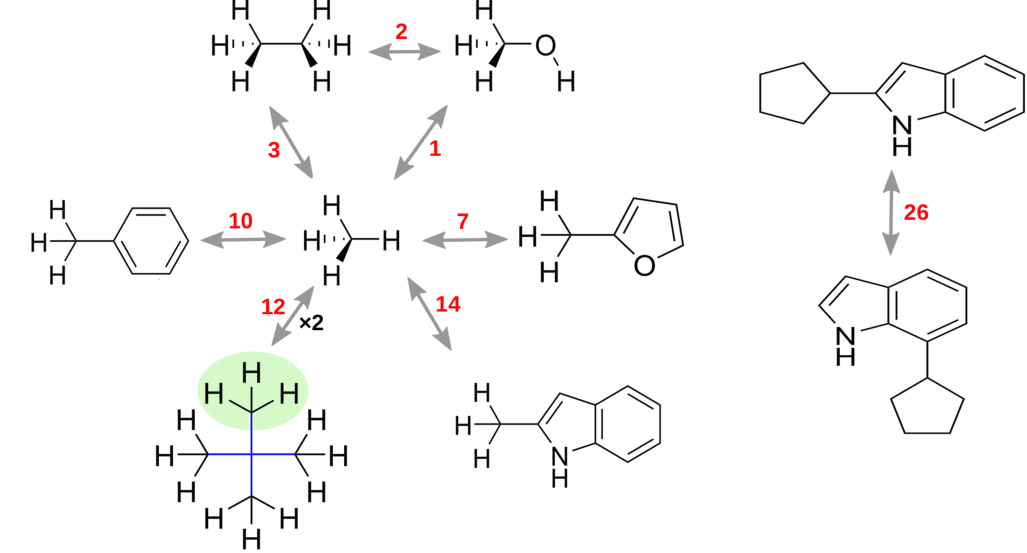
\includegraphics[scale=1.0]{figures/cycles.pdf}
  \caption{The thermodynamic cycles considered in this study.  To
    compute the free energy of hydration all pair--wise
    transformations have to be carried out once in solution and once
    in vacuum.  Green and blue colours in neopentane show two
    alternative mappings for methane.  The numbers in red denote the
    number of dummy atoms.}
  \label{fig:cycles}
\end{figure}
%DLM: Hannes, would you mind depositing PDFs with the figures compiled? I still 
%haven't been able to get the figures to compile properly locally, so it'd be 
%really useful if I could read a PDF that has the figures. :) 

The ethane $\rightarrow$ methanol transformation is traditionally
regarded as a standard test for RAFE
simulations~\cite{doi:10.1063/1.449208, doi:10.1021/jp981629f}.   The
other transformations are centered around mutations from and to
methane, and are meant to mimic typical transformations that could be attempted
in the context of e.g.\ protein-ligand binding calculations. The 
2--cyclopentanylindole to 7--cyclopentanylindole
transformation has been added to include both deletion as well as
insertion of sub--parts of the perturbed group in one simulation (in the 
following CPI will stand for cyclopentanylindole).  For
neopentane $\rightarrow$ methane we point out that there are two
alternative mappings possible, see Figure~\ref{fig:cycles}.  One in
which methane is mapped with a terminal methyl (green) and the other
one where the methane carbon is mapped with the central carbon in
neopentane (blue).  The first approach will be called ``terminally mapped'' and 
the second one ``centrally mapped''.


\subsection{RAFE Simulation Protocols}
\label{sec:rafe_protocols}

One of the major concerns in a reproducibility study is to ensure
consistency in the applied protocols.  This is complicated by the fact
that a given MD software may employ a wide range of methods and algorithms that
may not be available in other MD software.  For example, pressure and
temperature scaling, integrators and other algorithms can be very
different.  It is also unclear if and how implementation details can
affect results, in particular see subsection~\ref{sec:afe_impl} discussing the 
implementation details of alchemical free energy simulation in code.

In this study we look at a set of simple organic molecules (see
Figure~\ref{fig:cycles}).  As the focus here is on probing for
reproducibility among various MD packages, we chose fairly small,
rigid and neutral molecules to keep problems with sampling low, and
avoid difficulties with charged
particles~\cite{rocklin_calculating_2013, JCC:JCC1050}.  The force
field was chosen to be GAFF~\cite{wang_development_2004} (version
1.8), utilising AM1/BCC charges~\cite{jakalian_fast_2000,
  jakalian_fast_2002} for the solute and
TIP3P~\cite{jorgensen_comparison_1983-1} for the solvent.  Charges were 
computed with the \progname{antechamber} program and missing bonded and vdW 
terms were generated with the \progname{parmchk2} program, both from the 
AmberTools16 distribution.  The quality of free energies of various small 
molecule force fields has been shown
elsewhere, see e.g. Refs.~\citenum{doi:10.1021/ct300203w,Hu2016}.

While the MD packages principally allow a ``one--step'' 
transformation~\cite{steinbrecher_soft-core_2011}
that is both van der Waals and Coulombic softcore potentials vary
simultaneously, it can be more efficient to carry out a
separated protocol~\cite{naden_linear_2014, naden_linear_2015}. 
In such a protocol the charges are transformed
linearly between the end states followed by a mutation of the van der
Waals parameters using a softcore
potential~\cite{beutler_avoiding_1994,
  zacharias_separationshifted_1994} (see section~\ref{S-sec:softcores}x in the 
  SI for details) on the vdW
term only.  It is important to note that in the separated protocol
charges have to be switched off before vdW parameters (and vice versa
for the transformation in opposite direction) to avoid collapse of
other atoms, e.g. solvents, onto a ``naked'' charge, see 
section~\ref{S-sec:separated}x in the SI.
%DLM: I think there is a literature reference on the need to do this; asking 
%Guilherme for it as I don't recall it off the top of my head.

All simulations were started from the simulation box which has been 
created with FESetup~\cite{loeffler_fesetup:_2015}.  It should be noted, 
however, that in constructing the system steric overlaps between the solute and 
the solvent may happen.  This is because each unperturbed solute is 
independently equilibrated and the perturbed system combined from those two.  
The number of atoms are always chosen to be the same for forward and backward 
setups by using the larger box of the two unperturbed systems.  Thus, in 
transformation from a smaller to a larger solute water molecules may be in 
close distance to the solute.  The production simulations were run at 
\SI{298.15}{K} and \SI{1.0}{bar}.

\paragraph{AMBER} The starting coordinates were usually taken directly from the
pre--equilibrated setup step but no further $\lambda$ specific equilibration 
was carried out, i.e.\ RAFE MD simulations were started with new velocities 
appropriate for the 
final simulation temperature.  In a very few cases it was necessary to use 
coordinates from a nearby $\lambda$ state because of simulation instabilities.  
This happened in transformations with a larger number of dummy atoms.  Water 
hydrogens (TIP3P) were constrained with SHAKE but none of the atoms in the 
perturbed group and so the time step was set to \SI{1}{fs} (see SOMD protocol 
below for an alternative approach).  The temperature was controlled through a 
Langevin thermostat with a friction constant of \SI{2.0}{ps^{-1}} and pressure 
rescaling through a Monte Carlo barostat with 100 steps between isotropic 
volume change attempts.

\paragraph{CHARMM} The CHARMM c40b1 molecular dynamics package was used to 
carry out all relative hydration free energy simulations.  21 evenly spaced 
windows were used and all windows were run for \SI{1.5}{ns} with a timestep of 
\SI{1}{fs}.  Most windows used the same pre-equilibrated configuration, but a 
few windows were started with their own equilibration.  Constant temperature 
and pressure control was done with the Berendsen weak coupling method, with a 
compressibility of \SI{4.63e-5}{atm^{-1}} and temperature and pressure coupling 
constants of \SI{5.0}{ps^{-1}}.  A \SI{12.0}{\angstrom} atom--based cutoff was 
used for non--bonded interactions and Particle Mesh Eward (PME) with order of 6 
was used to calculate electrostatic forces along with periodic boundary 
condition.  SHAKE was used to constrain water hydrogens only.  The PERT module 
in CHARMM was used to handle alchemical transformation in conunction and PSSP 
softcore potential functions were used to avoid numerical issue at the end 
point lambdas.

\paragraph{GROMACS} We used GROMACS 4.6.7 to carry out simulations for 
the relative hydration free energies ($\Delta \Delta G_{\mathrm{hydr}}$).
Each transformation had its Gibbs free energy calculated: (i) in a single 
topology approach in which van der Waals energy terms were changed separately 
from the electrostatic and bonded components; (ii) in a single topology 
approach in which bonded, van der Waals, and electrostatic terms are changed 
together;  and (iii) via the difference between two absolute calculations.
In the first two cases, each alchemical transformation was described by 31 and 
16 states, respectively, and simulated for \SI{4.2}{ns} with time steps of 
\SI{1.0}{fs} in water and vacuum. Atomic masses were not changed along the 
alchemical path;
their change affect kinetic energy only and do not contribute to the free 
energy change on this case. 
We used the Langevin integrator implemented in GROMACS with a 
default friction coefficient of \SI{1.0}{ps/m_{atom}}. 
Absolute hydration free energies were calculated from \SI{5}{ns} Langevin 
dynamics
at \SI{298.15}{K}. We used the 20-step alchemical protocol where charge 
coupling and
van der Waals coupling were dealt with separately along the path 
\cite{Mobley2014, doi:10.1021/acs.jced.7b00104}.
%%JM: Elaborate a bit, especially regarding constraints
%%GDRM: Which sort of constraints do you think I should mention here?
%% From my mind I can't think of anything worth mentioning.
A Parrinello--Rahman barostat with $\tau_p =$ \SI{10}{ps} and compressibility 
equal to \SI{4.5d-5}{bar^{-1}}.
We used two methods to calculate electrostatic interactions: Particle Mesh 
Ewald (PME) and charge group-based Reaction Field with a dielectric of 78.3, 
as implemented in the software. 
%%JM : Please clarify if using an atom based or group based reaction field
We set the electrostatic and non--bonded cutoffs to \SI{10.0}{\angstrom};
a switch was applied to the latter starting at \SI{9.0}{\angstrom}. 
%%JM: switch applies to both RF and LJ ?
%% GDRM: LJ only. I'll clarify the text.
PME calculations were of order 6 and had a 
tolerance of \num{1.0d-6}, with a grid spacing of \SI{1.0}{\angstrom}. 
All transformations required the use of softcore potentials to avoid numerical 
problems in the free energy calculation.  We chose the 1--1--6 softcore 
potential for Lennard-Jones terms and used the default softcore Coulomb 
implementation in paths where charges, van der Waals, and bonded terms were 
modified together, but no soft core potentials were applied to Coulomb 
interactions when Coulomb interactions were modified separately.

\paragraph{SOMD} All simulations were carried out with
SOMD from the Sire 2016.1 release ~\cite{Sire-2016, doi:10.1021/ct300857j}
Each alchemical transformation was
divided into 17 evenly spaced windows and simulated for \SI{2}{ns}
both in water and in vacuum. A velocity-Verlet integrator was
employed with a \SI{2}{fs} time step, constraining only those hydrogen bonds
which are not alchemically transformed.  This approach will be called the 
``unperturbed protocol''. Referring to eq.~S\ref{S-eq:general-softcore}, 
the softcore parameters were set to default values for all the 
transformations, specifically $n = 0$ for Coulombic interactions and $\alpha = 
2.0$ for the Lennard-Jones potential.~\cite{doi:10.1021/ct700081t}
A shifted atom--based Barker--Watts reaction 
field~\cite{doi:10.1080/00268977300102101} with
a dielectric constant of \num{78.3} was adopted for the solution phase
simulations with a cutoff of \SI{10}{\angstrom}. A similar cutoff was used for 
Lennard-Jones interactions. Temperature control was achieved with the Andersen
thermostat~\cite{doi:10.1063/1.439486} with a coupling constant of
\SI{10}{ps^{-1}}.  A Monte Carlo barostat assured pressure control,
attempting isotropic box edge scaling every 25 time steps.
The reaction field was not employed in the vacuum legs, where a Coulombic 
potential without 
cutoff was used.  This leads to an inconsistent description of the 
intramolecular electrostatic interactions of the solute in the solvated and 
vacuum phases.   To maintain a consistent description of intramolecular 
energetics across vacuum and water legs,
a free energy correction term $G_{\mathrm{c}}$ was  evaluated as detailed in 
Ref.~\citenum{Bosisio2016}).  The
$G_{\mathrm{c}}$ term was obtained via post-processing of the end state 
trajectories of each water phase simulation, using the Zwanzig 
relationship~\cite{zwanzig_high-temperature_1954}:
\begin{equation}
 \label{eq:ZwanzigDGfunc}
 G_{\mathrm{c}} = -\beta^{-1} \ln \langle exp 
 \left[-\beta(U_{\mathrm{ic,nc}}(\mathbf{r}) - 
 U_{\mathrm{ic,sim}}(\mathbf{r}))\right]\rangle_{\mathrm{sim}}
\end{equation}
where $U_{\mathrm{ic,nc}}(\mathbf{r})$ is the solute intramolecular 
electrostatic-no cutoff 
potential that depends on the coordinates $\mathbf{r}$ of the solute and is 
given by Coulomb's law computed without cutoffs. 
$U_{\mathrm{ic,sim}}(\mathbf{r})$ is the intramolecular electrostatic potential 
term as
computed in the simulation with the shifted atom-based Barker-Watts Reaction 
Field cutoff.

To compute absolute free energy of hydration a double annihilation 
technique~\cite{jorgensen1988efficient,GILSON19971047,Bosisio2016}
was adopted. 
Initially the solute atoms' partial charges are turned off both in water and in 
vacuum, discharging step, giving a discharging
free energy change $\Delta G_\mathrm{solv}^\mathrm{elec}$ and $\Delta 
G_\mathrm{vac}^\mathrm{elec}$ respectively. Secondly,
the molecule is fully decoupled from the surrounding environment by switching 
off the van der Waals terms, vanishing step, retrieving a $\Delta 
G_\mathrm{solv}^\mathrm{vdW}$ in water phase and $\Delta 
G_\mathrm{vac}^\mathrm{vdW}$ in vacuum. 
Eventually, the absolute free energy of hydration $\Delta G$ can be computed as:
\begin{equation}
\label{eq:absolutehyd}
\Delta G = (\Delta G_\mathrm{solv}^\mathrm{elec} + \Delta 
G_\mathrm{solv}^\mathrm{vdW}) - (\Delta G_\mathrm{vac}^\mathrm{elec} + \Delta 
G_\mathrm{vac}^\mathrm{vdW})
\end{equation}
The same setup for relative free energy calculations was followed to compute 
absolute free energy of hydration. Thus, 17 evenly spaced $\lambda$ windows 
were used and simulations were run for \SI{2}{ns} employing a velocity-Verlet 
integrator with \SI{2}{fs} time step, constraining only the hydrogen bonds 
which are not alchemically transformed. 


\subsection{Analysis}
\label{sec:analysis}

Various estimators have been proposed to obtain the free energy from AFE 
simulations.  Early work by Kirkwood~\cite{kirkwood_statistical_1935} expresses 
the free energy as an ensemble average of the derivative of the
Hamiltonian with respect to the coupling parameter $\lambda$.  The
method is now known as Thermodynamic Integration (TI).  Zwanzig
devised the exponential formula~\cite{zwanzig_high-temperature_1954}
(EXP), also known as Free Energy Perturbation (FEP) or thermodynamic
perturbation (TP), which calculates the free energy from the
exponential average of the energy difference of the end states.  The
energy difference is computed from the energy with the configuration of one end 
state and reusing it to compute the energy with the force field parameters of 
the other end state.  This obviously assumes that the configuration is
representative of both state.  As the phase--space overlap needs to
be sufficiently large~\cite{wu_phase-space_2005,
  wu_phase-space_2005-1} the EXP approach typically needs
intermediates, controlled by $\lambda$.  However, it has been shown
that EXP has an asymmetric bias depending on the directionality of
$\lambda$~\cite{wu_asymmetric_2004} and that the Bennett Acceptance
Ratio (BAR) method~\cite{bennett_efficient_1976} is considerably more
effective in obtaining an accurate result~\cite{lu_appropriate_2003}.
BAR is a generalization of EXP by making explicit use of the
``forward'' ($\lambda_i \rightarrow \lambda_{i+1}$) and ``backward''
($\lambda_{i+1} \rightarrow \lambda_i$) estimates.  Later it was
demonstrated that this can be effectively extended to incorporate all
other $\lambda$s.  This approach has been called multi--state BAR
(MBAR)~\cite{shirts_statistically_2008-1}.  MBAR has been shown
to have the lowest variance of any known
estimator~\cite{shirts_statistically_2008}.
%JM I don't think we need all of this at this stage of the paper, go straight to
%TI and justify why we use it.
% HHL: can go to Discussion under the title of ``recommendations''

In this work we primarily focus on TI as this is supported by all MD
packages ``out--of--the--box'', whereas BAR and MBAR are not.
Equation~\ref{eq:ti} computes the free energy as
\begin{equation}\label{eq:ti}
	\Delta G = \int_{\lambda=0}^{\lambda=1}
	\left\langle 
	\frac{\mathscr{H}(\vec{q},\vec{p};\lambda)}{\partial\lambda}\right\rangle_\lambda
	 d\lambda
\end{equation}
where $\mathscr{H}(\vec{q},\vec{p};\lambda)$ is the Hamiltonian as a function 
of the coordinate vectors $\vec{q}$ and the momentum vectors $\vec{p}$, and 
parametric dependence on the coupling parameter $\lambda$.  The angle brackets 
denote the ensemble average of the gradient of the Hamiltonian with respect to 
$\lambda$ at a given $\lambda$ value.  An AFE simulation is typically carried 
out in a series of equilibrium simulations at discrete values of $\lambda$ but 
the gradient can also be evaluated with a continuously varying coupling 
parameter as a function of the simulation time.  The free energy is finally 
computed through a suitable numerical integration method.
%%JM We don't actually compute momenta contribution in the codes so needs 
%%clarification. Also since this justifies 
%%changing masses of elements (which FESetup does), we should delve on that. 

Results from additional estimators
will be given where available.  We have used the alchemical analysis
tool~\cite{klimovich_guidelines_2015} for analysis of all free energies.  This
tool provides various estimators such as TI, TI with cubic splines,
BAR and MBAR.  All data can be sub--sampled to eliminate correlated
data.

All RAFE simulations were run in triplicate in forward as well as
backward direction for a total of 6 simulations per mutation.  The
final hydration free energy $\Delta\Delta G_{\mathrm{hydr}}$ was
computed as the average for each direction separately.  For comparison we have 
also calculated the absolute (standard) hydration free energies for all
molecules in Figure~\ref{fig:cycles}.  These energies are less 
implementation--dependent and thus provide an additional check.
%%JM remove this sentence and discuss the finding (less implementation dependent
%%in the results section)

To estimate the reliability and convergence of the results, the
standard error of the mean (SEM) has been calculated.  The SEM is
defined as

\begin{equation}
  \label{eq:sem}
  \mathrm{err}(\Delta\Delta G_{\mathrm{hydr}}) = \frac{\sigma}{\sqrt{n}}
\end{equation}

where $\sigma$ is the sample standard deviation and $n$ is the size of
the uncorrelated sample.  The SEM for component free energies is combined as

\begin{equation}
  \label{eq:sem-comb}
  \mathrm{err}(\mathrm{combined}) = \sqrt{\sum_i \sigma_i^2}.
\end{equation}

which is appropriate if the property to be computed is a sum of
contributions.

We also make use of the mean absolute error MAE (also called mean unsigned 
error, MUE) to compare data sets.
\begin{equation}
\label{eq:MUE}
\mathrm{MAE} = \frac{1}{n}\sum_\mathrm{i=1}^n \left | y_\mathrm{i} - 
x_\mathrm{i} \right |
\end{equation}
where $n$ is the total number of samples, $y_\mathrm{i}$ and $x_\mathrm{i}$ are 
the $i$--th datum to be compared.


\section{Results}
\label{sec:results}

We will use absolute hydration free energies here as our standard point of 
comparison because these are easily calculated with considerable precision
\cite{doi:10.1021/acs.jced.7b00104} %check for more references
and are considerably simpler to set up and implement than relative calculations.
Prior work actually compared calculated absolute hydration free energies across 
different codes with considerable success~\cite{klimovich_predicting_2010} (see 
Fig.~7 in the reference), further supporting this view.

Thus, we compare relative free energies calculated via simultaneous parameter 
change simulations --- our ``unified protocol'' --- and separated parameter 
change simulations --- our ``split protocol''--- to relative free energy 
calculations obtained from two absolute hydration free energies -- our 
``absolute protocol''.
% HHL: GDRM, is the absolute protocol a unified or a split protocol?  For
%      AMBER, CHARMM and SOMD it is a unified protocol.
% GDRM: Yes, it is
The unified protocol changes partial charges, van der Waals parameters, and 
bond parameters simultaneously along the alchemical path, while the split 
protocol separates the transformation of the van der Waals parameters from the 
charge transformation.  The order in which this has to be done is detailed 
in section~\ref{S-sec:separated}x of the SI.  The scaling of the bonded terms 
can be combined with either transformation.

Table~\ref{tab:absolute} summarizes results for relative free energies of 
hydration obtained from absolute transformations.  The table shows the data 
from simulations with the recommended protocol as discussed in detail in the 
following subsections for each MD code. The $\Delta\Delta G_{\mathrm{hydr}}$ 
obtained with the various MD packages in 
this way agree quite well, although some larger deviations are apparent as 
well.  GROMACS predicts a smaller $\Delta\Delta G_{\mathrm{hydr}}$ for the 
methanol transformations by about \SI{0.2}{kcal.mol^{-1}}.  Similarly, there 
are some discrepancies in the toluene, 2--methylfuran and 2--methylindole cases 
where it is mostly CHARMM that produces somewhat smaller $\Delta\Delta 
G_{\mathrm{hydr}}$ with \SI{0.4}{kcal.mol^{-1}} difference between the 
smallest and highest values.  The largest deviation can be found in the largest 
transformation where the AMBER result is higher by 0.4--\SI{0.5}{kcal.mol^{-1}} 
than the other MD packages.
%SB: Why don't we consider Gromacs Reaction Field here ?
% HHL: we present here only the recommended protocol
\begin{table}[]
  \begin{minipage}{\linewidth}
    \caption{Comparing relative free energies of hydration for various MD 
    packages as obtained from absolute transformations.}\label{tab:absolute}
    \makebox[\textwidth][c]{
      \begin{tabular}{llrrrr}
        \toprule
        \multicolumn{2}{l}{transformation} & 
        AMBER\footnote{\label{foot:unified}unified protocol.} & 
        CHARMM\footref{foot:unified} & GROMACS\footnote{split protocol with 
        PME.} & SOMD\footref{foot:unified}
        \\
        \midrule
        ethane & methane & \num{-0.02+-0.01} & \num{-0.08+-0.01} & \num{-0.04 
        +- 0.01} & \num{-0.05+-0.02} \\
        methanol & methane & \num{6.20+-0.01} & \num{6.15+-0.02} & \num{5.95 +- 
        0.01} & \num{6.21+-0.06} \\
        ethane & methanol & \num{-6.22+-0.01} & \num{-6.23+-0.02} & \num{-5.98 
        +- 0.01} & \num{-6.26+-0.05} \\
        toluene & methane & \num{3.19+-0.01} & \num{3.00+-0.01} & \num{3.16 +- 
        0.01} & \num{3.07+-0.03} \\
        neopentane & methane & \num{-0.13+-0.02} & \num{-0.18+-0.02} & 
        \num{-0.14 +- 0.01} & \num{-0.19+-0.06} \\
        2--methylfuran & methane & \num{2.96+-0.02} & \num{2.79+-0.01} & 
        \num{2.95 +- 0.01} & \num{2.90+-0.03} \\
        2--methylindole & methane & \num{8.72+-0.01} & \num{8.36+-0.02} & 
        \num{8.79 +- 0.02} & \num{8.57+-0.03} \\
        2--CPI & 7--CPI & \num{0.39+-0.04} & \num{-0.10+-0.04} & \num{0.02 +- 
        0.05} & \num{0.08+-0.14} \\
        \bottomrule
      \end{tabular}
    }
  \end{minipage}
\end{table}

Tab~\ref{tab:mue-absolute} shows the MAE between SOMD, GROMACS, AMBER and 
CHARMM.
%(alternatively: Tab~\ref{tab:muebound-comp} shows the MAE comparison with a
%95$\%$ confidence interval). 
The MAE appears to be fairly small generally and reaches just about 
\SI{0.2}{kcal.mol^{-1}} between CHARMM and GROMACS, and CHARMM and AMBER.
\begin{table}[]
  \begin{minipage}{\linewidth}
    \caption{MAE (\SI{}{kcal.mol^{-1}}) comparing relative free energies from 
      absolute simulations between SOMD, GROMACS, AMBER and 
      CHARMM.}\label{tab:mue-absolute}
    \makebox[\textwidth][c]{
      \begin{tabular}{lrrr}
        \toprule
        Package & GROMACS & AMBER & CHARMM\\
        \midrule
        SOMD    & 0.12 & 0.09 & 0.08 \\
        GROMACS &      & 0.13 & 0.17 \\
        AMBER   &      &      & 0.16 \\
        \bottomrule
      \end{tabular}
    }
  \end{minipage}
\end{table}

Having established the predictions from absolute transformations we now turn to 
computing $\Delta\Delta G_{\mathrm{hydr}}$ from relative mutations.  
Table~\ref{tab:relative} summarizes the results for the four MD packages.  
Again the data is from the recommended protocol (see detailed discussions in 
the following subsections).
\begin{table}[]
  \begin{minipage}{\linewidth}
    \caption{Comparing relative free energies of hydration for various MD 
      packages as obtained from relative transformations.  Signs of the 
      backward transformation have been reverted to correspond to the forward 
      transformation.}\label{tab:relative}
    \makebox[\textwidth][c]{
      \begin{tabular}{llrrrrr}
        \toprule
        & & \multicolumn{2}{c}{AMBER} & CHARMM & GROMACS & SOMD \\
        & & \multicolumn{1}{c}{implicit} & \multicolumn{1}{c}{explicit} & & & \\
        \midrule
        ethane & methane & \num{0.02+-0.01} & \num{-0.13+-0.02} & \num{-0.11 +- 
        0.02} & \num{-0.04 +- 0.02} & \num{-0.01+-0.05} \\
        methane & ethane & \num{0.00+-0.03} & \num{-0.19+-0.03} & \num{-0.06 +- 
        0.01} & \num{-0.02 +- 0.01} & \num{-0.04+-0.02} \\
        methanol & methane & \num{6.19+-0.01} & \num{6.20+-0.02} & \num{6.17 +- 
        0.01} & 
        \num{6.20 +- 0.01} & \num{5.99+-0.05} \\
        methane & methanol & \num{6.20+-0.03} & \num{6.15+-0.01} & \num{6.20 +- 
        0.01} & \num{6.20 +- 0.01} & \num{5.96+-0.04} \\
        ethane  & methanol & \num{-6.20+-0.01} & \num{-6.27+-0.01} & \num{-6.26 
        +- 0.01} & \num{-6.19 +- 0.01} & \num{-6.09+-0.03} \\
        methanol & ethane & \num{-6.20+-0.01} & \num{-6.25+-0.01} & \num{-6.29 
        +- 0.01} & \num{-6.19+- 0.01} & \num{-6.09+-0.02} \\
        toluene & methane & \num{3.24+-0.02} & \num{3.39+-0.02} & \num{2.93 +- 
        0.02} & \num{3.21 +- 0.01} & \num{2.89+-0.09} \\
        methane & toluene & \num{3.42+-0.03} & \num{3.52+-0.03} & \num{2.96 +- 
        0.02} & \num{3.20 +- 0.01} & \num{3.06+-0.02} \\
        neopentane\footnote{\label{foot:cent}central mapping.} & methane & 
        \num{0.32 +-0.04} & \num{-0.03+-0.06} & \num{-0.44 +- 0.01} & 
        \num{-0.15 +- 0.02} & \num{-0.20+-0.05} \\
        methane\footref{foot:cent} & neopentane & \num{0.25+-0.03} & 
        \num{-0.07+-0.03} & \num{-0.33 +- 0.02} & \num{-0.16 +- 0.05} & 
        \num{-0.13+-0.05} \\
        neopentane\footnote{\label{foot:term}terminal mapping.} & methane & 
        \num{-0.13+-0.01} & \num{-0.12+-0.02} & \num{-0.65 +- 0.02} & 
        \num{-0.14 +- 0.01} & \num{-0.11+-0.01} \\
        methane\footref{foot:term} & neopentane & \num{-0.13+-0.03} & 
        \num{-0.12+-0.03} & \num{-0.49 +- 0.02} & \num{-0.18 +- 0.03} & 
        \num{-0.10+-0.06} \\
        2--methylfuran  & methane & \num{3.09+-0.01} & \num{3.10+-0.01} & 
        \num{2.76 +- 0.03} & \num{2.93 +- 0.05} & \num{2.92+-0.05} \\
        methane & 2-methyfuran  & \num{3.10+-0.03} & \num{3.15+-0.03} & 
        \num{2.76 +- 0.02} & \num{2.96 +- 0.01} & \num{2.83+-0.03} \\
        2--methylindole & methane & \num{8.78+-0.03} & \num{8.78+-0.04} & 
        \num{8.34 +- 0.01} & \num{8.73 +- 0.03} & \num{8.64+-0.06} \\
        methane & 2-methylindole & \num{9.14+-0.02} & \num{9.13+-0.03} & 
        \num{8.42 +- 0.02} & \num{8.74 +- 0.01} & \num{8.67+-0.08} \\
        2--CPI\footnote{\label{foot:partial}partial 
        re/discharge i.e.\ only the charges of the appearing and the 
        disappearing 5--rings are switched.} & 7--CPI & 
        \num{0.36+-0.03} & \num{0.63+-0.06} & \num{-0.01 +- 0.01} & \num{-0.03 
        +- 0.03} & \num{-0.11+-0.07} \\
        7--CPI\footref{foot:partial} & 2--CPI & 
        \num{0.34+-0.05} & \num{0.50+-0.03} & \num{0.03 +- 0.01} & \num{-0.20 
        +- 0.04} & \num{-0.01+-0.08} \\
        \bottomrule
      \end{tabular}
    }
  \end{minipage}
\end{table}

Overall, the predicted $\Delta\Delta G_{\mathrm{hydr}}$ valued from the four MD 
packages are in good agreement with each other.  CHARMM tends to show smaller 
relative free energies in a number of transformations: toluene, neopentane, 
2--methylfuran and 2--methylindole.  SOMD displays smaller $\Delta\Delta 
G_{\mathrm{hydr}}$ in the methanol and toluene transformations.  The largest 
discrepancy, however, is in the neopentane transformation with central mapping 
where AMBER with implicit dummy atoms is about \SI{0.5}{kcal.mol^{-1}} higher 
and CHARMM about \SI{0.3}{kcal.mol^{-1}} lower than the other two codes.  The 
terminal mapped neopentane reveals AMBER to be in line with GROMACS and SOMD 
while CHARMM's results is essentially the same as in the central mapped 
transformation.  AMBER deviates also quite strongly from the other codes in the 
cyclopentanyl indole cases.

The MAEs of the relative free energy simulations are presented in 
Table~\ref{tab:mue-relative}.  These are continuously larger than the MAEs from 
the absolute simulations (Table~\ref{tab:mue-absolute}) and reach 
\SI{0.3}{kcal.mol^{-1}} for CHARMM compared with AMBER and GROMACS.
\begin{table}[]
  \begin{minipage}{\linewidth}
    \caption{MAE (in \si{kcal.mol^{-1}}) comparing relative free energies from 
      relative simulations between SOMD, GROMACS, AMBER and 
      CHARMM.}\label{tab:mue-relative}
    \makebox[\textwidth][c]{
      \begin{tabular}{lrrr}
        \toprule
        Package & GROMACS & AMBER & CHARMM \\
        \midrule
        SOMD    & 0.18 & 0.23 & 0.19 \\
        GROMACS &      & 0.14 & 0.31 \\
        AMBER   &      &      & 0.32 \\
        \bottomrule
      \end{tabular}
    }
  \end{minipage}
\end{table}

%\begin{table}[]
%  \begin{minipage}{\linewidth}
%    \caption{MAE (\SI{}{kcal.mol^{-1}})with 95$\%$ confidence interval between 
%SOMD, GROMACS 
%    with 
%      Reaction Field (GROMACS RF), GROMACS with PME (GROMACS PME), AMBER and 
%CHARMM.}
%      \label{tab:muebound-comp}
%    \makebox[\textwidth][c]{
%      \begin{tabular}{lccccc}
%        \toprule
%        Package & SOMD & Gromcs RF & GROMACS PME & AMBER & CHARMM\\
%        \midrule
%        SOMD         & 0.02< 0.04< 0.05 & 0.17< 0.19< 0.21    & 0.16< 
%        0.18< 0.20 & 0.21< 0.23< 0.25 & 0.18< 0.19< 0.20\\
%        GROMACS RF   	  & 0.17< 0.18< 0.19 & 0.01< 0.02< 0.03    & 0.04< 
%0.05< 
%        0.06 & 
%        0.13< 0.14< 0.15 & 0.31< 0.32< 0.33\\
%        GROMACS PME       & 0.17< 0.18< 0.19 & 0.04< 0.05< 0.06    & 0.01< 
%        0.02< 0.03 & 
%        0.14< 0.15< 0.16 & 0.30< 0.31< 0.32\\
%        AMBER		  & 0.22< 0.23< 0.24 & 0.13< 0.14< 0.15    & 0.14< 0.15< 0.16 
%& 
%        0.01< 
%        0.02< 0.03 & 0.31< 0.32< 0.33\\
%        CHARMM & 0.17< 0.19< 0.21 & 0.31< 0.32< 0.33 & 0.30< 0.31< 0.32 & 
%0.31< 0.32< 0.33 & 0.01< 0.02 <0.03\\
%        \bottomrule
%      \end{tabular}
%    }
%  \end{minipage}
%\end{table}

%\begin{table}[]
%  \begin{minipage}{\linewidth}
%    \caption{MAE (\SI{}{kcal.mol^{-1}}) with 95$\%$ confidence interval 
%between SOMD, GROMACS 
%    with 
%      Reaction Field (GROMACS RF), GROMACS with PME (GROMACS PME), AMBER and 
%CHARMM for relative
%      free energy prediction computed with the absolute 
%protocol}\label{tab:muebound-abs}
%    \makebox[\textwidth][c]{
%      \begin{tabular}{lccccc}
%        \toprule
%        Package & SOMD & Gromcs RF & GROMACS PME & AMBER & CHARMM\\
%        \midrule
%        SOMD         & 0.02< 0.04< 0.06 & 0.15< 0.16< 0.18    & 0.11< 
%        0.12< 0.14 & 0.08< 0.09< 0.10 &0.07< 0.08< 0.09\\
%        GROMACS RF   	  & 0.15< 0.16< 0.17 & 0.01< 0.02< 0.03    & 0.12< 
%0.13< 
%        0.14 & 
%        0.23< 0.24< 0.25 & 0.12< 0.13< 0.14\\
%        GROMACS PME       & 0.11< 0.13< 0.16 & 0.13< 0.14< 0.15    & 0.01< 
%        0.02< 0.03 & 
%        0.11< 0.12< 0.13 & 0.15< 0.16< 0.18\\
%        AMBER		  & 0.07< 0.10< 0.13 & 0.23< 0.24< 0.25    & 0.11< 0.12< 0.13 
%& 
%        0.01< 
%        0.02< 0.03 & 0.15< 0.16< 0.18\\
%        CHARMM & 0.07< 0.08< 0.09 & 0.12< 0.13< 0.14 & 0.15< 0.17< 0.18 & 
%0.15< 0.16 <0.17 & 0.01<0.02<0.03\\
%        \bottomrule
%      \end{tabular}
%    }
%  \end{minipage}
%  \end{table}


\subsection{AMBER}
\label{sec:amber-results}

Using AMBER for RAFE simulations has revealed several problems with
the implementation.  Some bugs were identified and have been fixed for AMBER16 
release by the developers, e.g. energy minimization in \progname{sander} led to 
diverged coordinates for mapped atoms.  For a single topology description, 
however, it is necessary to have the same coordinates.  Other issues are that 
vacuum simulations can only be carried out with the \progname{sander} program 
because \progname{pmemd} cannot handle AFE simulations in vacuum at the 
moment.  This will, however, be rectified in future 
versions~\cite{doi:10.1021/acs.jctc.7b00102}.  A disadvantage of 
\progname{sander} is that it cannot be used to simulate the $\lambda$ end 
points~\cite{doi:10.1021/ct400340s} such that the TI gradients need to be 
extrapolated (minimum and maximum allowed $\lambda$s are 0.005 and 0.995). 
%DLM: Wait, so this means that there's no way around extrapolating the 
%endpoints in vacuum?
%HHL: Yes, extrapolation needs to be done with sander.
 Also, \progname{sander} considers the whole system as the perturbed
region while \progname{pmemd} restricts this to a user chosen atom selection.  
This
has obvious implications for performance~\cite{doi:10.1021/ct400340s}.

We also found that, in contrast to the other three codes, AMBER cannot
correctly reproduce relative free energies in the unified protocol i.e.\
when all force field parameters are scaled simultaneously (see 
Table~\ref{S-tab:amber-onestep}x).  This appears to be a problem when more than 
a few dummy atoms are involved while the unified protocol works for the smaller 
transformations (refer to Figure~\ref{fig:cycles}).  The separated RAFE 
protocol and absolute free energies, however, are very close to the other MD 
packages as demonstrated in Table~\ref{tab:amber-comp}.

End point geometries appear to be another issue with AMBER simulations
in both solution and vacuum.  This is most obvious in the neopentane 
$\rightarrow$ methane test case with central mapping (see 
\nameref{sec:rafe_setup} and Figure~\ref{fig:thermocycle}).
As shown in Figure~\ref{S-fig:amber-dist}x, the methane end state exhibits 
incorrect distances between the carbon and the four 
attached hydrogens of approximately \SI{1.23}{\angstrom}.  This value is about 
\SI{1.12}{\angstrom} for the terminal dummy atoms in the other test cases but 
still higher than the expected \SI{1.09}{\angstrom} on average.  
Figure~\ref{S-fig:amber-dist}x demonstrates how this depends on the number of 
dummy atoms immediately surrounding the central atom.
%DLM: I think we need error bars on the values otherwise it's impossible to 
%tell if the difference is significant.
%HHL: We can also compare this between all MD codes.  I'm confident this is 
%significant.

We also compare free energies obtained from the implicit dummy approach in 
AMBER with results form explicit dummy atom simulations and results from 
absolute transformations, see Tables~\ref{tab:absolute} and 
\ref{tab:relative}.  The relative simulations have been carried out with the 
separated protocol while the absolute simulations used a unified protocol 
throughout.  SHAKE was explicitly deactivated for all bonds in the perturbed 
region in these protocols.

Table~\ref{tab:amber-comp} shows selected results for transformations with 
SHAKE enabled for all bonds to hydrogens except those bonds that change bond 
length during transformation. 
\begin{table}[]
  \begin{minipage}{\linewidth}
  \caption{Comparing AMBER results for simulations with various protocols.
    The emphasis is here on the data with SHAKE enabled and a time step of 
    \SI{2}{fs} (last column).  Implicit, explicit and absolute protocols had 
    SHAKE disabled and a time step of \SI{1}{fs}. Signs of the  backward 
    transformation have been reverted to correspond to the forward   
    transformation.}\label{tab:amber-comp}
  \makebox[\textwidth][c]{
  \begin{tabular}{llrrrr}
    \toprule
    &                & implicit & explicit & absolute & SHAKE\footnote{implicit 
    dummy atom protocol with $\delta t =$ \SI{2}{fs} and SHAKE on all H--bonds 
    except perturbed bonds.} \\
    \multicolumn{2}{l}{transformation}          & $\Delta\Delta G$  & 
    $\Delta\Delta G$ & $\Delta G$ & $\Delta\Delta G$ \\
    \midrule
ethane  & methanol & \num{-6.20+-0.01} & \num{-6.27+-0.01} &
\multirow{2}{*}{\num{-6.22+-0.01}} & -6.20 \\
methanol & ethane & \num{-6.20+-0.01} & \num{-6.25+-0.01} & & \\
toluene & methane & \num{3.24+-0.02} & \num{3.39+-0.02} &
\multirow{2}{*}{\num{3.19+-0.01}} & 3.29 \\
methane & toluene & \num{3.42+-0.03} & \num{3.52+-0.03} & & \\
neopentane\footnote{\label{foot:centA}central mapping.} & methane & \num{0.32 
+-0.04} & \num{-0.03+-0.06} & \multirow{4}{*}{\num{-0.13+-0.02}} & 0.37 \\
methane\footref{foot:centA} & neopentane & \num{0.25+-0.03} & \num{-0.07+-0.03} 
& & \\
neopentane\footnote{\label{foot:termA}terminal mapping.} & methane & 
\num{-0.13+-0.01} & \num{-0.12+-0.02} & & \\
methane\footref{foot:termA} & neopentane & \num{-0.13+-0.03} & 
\num{-0.12+-0.03} 
& & \\
    \bottomrule
  \end{tabular}
}
  \end{minipage}
\end{table}
These free energies are computed from a single 
run as we generally observe very small SEM and in practice one simulation is 
sufficient to obtain converged free energy averages for all the systems studied 
here.  The time step has been increased from \SI{1}{fs} as used in the other 
three protocols to \SI{2}{fs}.  As the results are essentially the same as the 
non--SHAKE simulations, this SHAKE protocol appears to be a viable solution to 
increase the performance of RAFE simulations.  We have repeated this protocol 
with AMBER in response to the good results obtained with SOMD using the same.  
From a practical point of view, 
%DLM: How much speed difference does this make?
%HHL: I would say by a factor of two as the number of SHAKEs is practically the 
%same.
%JM: You could explicitly state that this protocol was tested in response to 
% the feedback from the SOMD calculations, we can spin this then as a benefit 
% of having developers talk to each other :-) 
AMBER uses an \emph{atom} based mask for bond SHAKEs such that the mask must be 
set for the hydrogens in question while the same is not possible for their 
non--H counter--part in the other state because \emph{all} bonds emanating from 
this atom would be affected.

We can also compute the cycle closure error from Table~\ref{tab:amber-comp} for 
the closed cycle ethane$ \rightarrow$ methanol $\rightarrow$ methane 
$\rightarrow$ ethane (see Figure~\ref{fig:cycles}).  The free energy difference 
within a closed thermodynamic cycle must necessarily be zero.
%%JM sentence not necessary?
For the implicit dummy simulation we calculate a cycle error for $\Delta\Delta 
G_\mathrm{hydr}$ of \SI{0.069+-0.041}{kcal.mol^{-1}} and for the explicit dummy 
simulation the error is \SI{-0.016+-0.047}{kcal.mol^{-1}}.

In general, the free energies computed with each approach are in good agreement 
with each other and with the results of the other MD packages.  There are, 
however, a few notable deviations.  Neopentane $\rightarrow$ methane with 
central mapping differs from the result with terminal mapping by about 
\SI{0.4}{kcal.mol^{-1}} (cf.\ Table~\ref{tab:amber-comp}).
The terminal mapping and the free energies from the explicit dummy simulations 
are, however, consistent with the absolute transformations.  We also observe a 
systematic deviation between forward and backward vacuum transformations in 
particular in the 2--methylindole simulation (see Table~\ref{S-tab:amber-disc}).
A discrepancy of consistently 0.2--\SI{0.4}{kcal.mol^{-1}} is evident from 
every $\lambda$ step of the vdW plus bonded transformation with both implicit 
and explicit dummy atoms).
%%JM: any hint of the problem? This suggests a bug in AMBER
% HHL: no hints yet, only symptoms.  Strongly suspect a bug too.

\subsection{CHARMM}
\label{sec:charmm-results}

\todo{bug in TI gradient accumulation in parallel runs (does not affect
	serial?, does not affect EXP)}

\todo{cannot handle LRC: test with larger cutoffs and/or LRC correction
	with arbitrary, single structure; check 
	http://pubs.acs.org/doi/abs/10.1021/jp0735987}

\subsection{GROMACS}
\label{sec:gromacs-results}

GROMACS has some run input options which can simplify the procedure 
for setting up free energy calculations.  Specifically, \inpopt{couple-moltype} 
implicitly defines the initial and final states by giving a special tag to a 
molecule and controls whether intramolecular interactions of the tagged 
molecule are retained or not along the alchemical path.  It should be used in 
absolute free energy calculations to tag the molecule which will be decoupled 
from the rest of the system.  \inpopt{couple-lambda0} and 
\inpopt{couple-lambda1} control the interactions of the molecule specified by 
\inpopt{couple-moltype} with its surroundings.
The entries \inpopt{vdw-lambdas} and \inpopt{fep-lambdas} 
define the lambda schedule.  The former indicates the value of the $\lambda$ 
vector component that modifies van der Waals interactions for each state,
while the latter changes all $\lambda$ vector components that are not specified 
in the \inpopt{.mdp} file.  For instance, in split protocol simulations, these 
entries are sets such that the components of the energy are modfied in 
different stages.  If the transformation involves particle deletion ("forward 
process"), \inpopt{fep-lambdas} is set to change charges and bonds
before \inpopt{vdw-lambdas} changes van de Waals components.
If the process involves particle insertion ("backward process") we reverse 
the roles.  In this work, \inpopt{mass-lambdas} were all set to zero  to not 
included mass changes in the free energy.  Unified protocols set all $\lambda$ 
vectors the same.

%JM: Do you have a way to control the strength of softening of Coul and LJ in 
%Gromacs?
% Does the soft-core apply to ALL atoms, or only atoms that are dummies in one 
%end-state?
% We must delve in differences with the SOMD softcore for the discussions 
%section.

% GDRM: What do you mean by "control the strength of softening ..."? 
%     The user is given the opportunity to choose if he/she wants to use
%     soft-core potentials and to choose its parameters (power, alpha and 
%sigma).
%     Regarding sc potentials, I'm inclined to say they are applied to all 
%atoms, but
%     I'm not sure about it. I've checked the documentation and it is not clear 
%as well.
%     Perhaps I should check the code; I'll have this answered in a future pull 
%request.
% HHL: IIRC Michael Shirts said that LJ softcores are applied when the 
%      LJ parameter(s) (don't recall which) are zer0

Table \ref{tab:groresults} lists the relative free energies obtained from 
GROMACS simulations.
\begin{sidewaystable}[]
  \centering
  \caption{Relative hydration free energies obtained from GROMACS simulations 
  in $kcal\cdot mol^{-1}$. Signs of the backward transformation have been 
  reverted
  to correspond to the forward transformation.}
  \label{tab:groresults}
  \resizebox{\columnwidth}{!}{%
    \begin{tabular}{@{}rrrrrrrr@{}}
    \toprule
    &  & \multicolumn{2}{c}{split\footnote{results obtained 
    from alchemical transformations with electrostatic and bonded scaling 
    separate from vdW  parameter change.}} & 
    \multicolumn{2}{c}{unified\footnote{results obtained from 
    alchemical transformation 
    with all parameters scaling together.}} & 
    \multicolumn{2}{c}{absolute\footnote{results obtained from 
    absolute free energy 
    calculations.}} \\
    \multicolumn{1}{c}{} & \multicolumn{1}{c}{} & \multicolumn{1}{c}{RF} & 
    \multicolumn{1}{c}{PME} & \multicolumn{1}{c}{RF} & \multicolumn{1}{c}{PME} 
    & \multicolumn{1}{c}{RF} & \multicolumn{1}{c}{PME} \\
    \multicolumn{2}{c}{transformation} & \multicolumn{1}{c}{$\Delta \Delta G$} 
    & \multicolumn{1}{c}{$\Delta \Delta G$} & \multicolumn{1}{c}{$\Delta \Delta 
    G$} & \multicolumn{1}{c}{$\Delta \Delta G$} & \multicolumn{1}{c}{$\Delta 
    \Delta G$} & \multicolumn{1}{c}{$\Delta \Delta G$} \\ \midrule
    ethane & methane & \num{-0.03 +- 0.01} & \num{-0.04 +- 0.02} & 
    \num{-0.02+- 0.00} & \num{-0.03 +- 0.00} & \num{-0.06 +- 0.01} & 
    \num{-0.04 +- 0.01} \\
    methane & ethane & \num{-0.01 +- 0.02} & \num{-0.02 +- 0.01} & \num{0.046 
    +- 0.02}\footnote{\label{foot:inv} inverted sign} & \num{0.01 +- 0.02} &  
    &  \\
    methanol & methane & \num{6.16 +- 0.01} & \num{6.20 +- 0.00} & 
    \num{7.30 +- 0.02} & \num{7.38 +- 0.01} & \num{5.77 +- 0.01} & \num{5.95 
    +- 0.01} \\
    methane & methanol & \num{6.17 +- 0.01} & \num{6.20 +- 0.01} & 
    \num{7.09 +- 0.02} & \num{7.17 +- 0.02} &  &  \\
    ethane & methanol & \num{-6.12 +- 0.01} & \num{-6.19 +- 0.01} & 
    \num{-7.12 +- 0.01} & \num{-7.21 +- 0.02} & \num{-5.83 +- 0.01} & 
    \num{-5.98 +- 0.01} \\
    methanol & ethane & \num{-6.12 +- 0.01} & \num{-6.19+- 0.00} & 
    \num{-7.34 +- 0.00} & \num{-7.40 +- 0.00} &  &  \\
    toluene & methane & \num{3.22 +- 0.01} & \num{3.21 +- 0.01} & \num{3.23 
    +- 0.01} & \num{3.22 +- 0.01} & \num{2.97 +- 0.01} & \num{3.16 +- 0.01} \\
    methane & toluene & \num{3.25 +- 0.01} & \num{3.20 +- 0.01} & \num{3.22 +- 
    0.01} & \num{3.21 +- 0.00} &  &  \\
    neopentane\footnote{\label{foot:c-map}central mapping} & methane & 
    \num{-0.10 +- 0.01} & \num{-0.15 +- 0.02} & \num{-0.08 +- 0.02} & 
    \num{-0.18 +- 0.03} & \num{-0.18 +- 0.01} & \num{-0.14 +- 0.01} \\
    methane\footref{foot:c-map} & neopentane & \num{-0.11 +- 0.02} & \num{-0.16 
    +- 0.05} & \num{0.00 +- 0.03} & \num{-0.18 +- 0.03} &  &  \\
    neopentane\footnote{\label{foot:t-map}terminal mapping} & methane & 
    \num{-0.12 +- 0.01} & \num{-0.13 +- 0.01} & \num{-0.14 +- 0.01} & 
    \num{-0.14 +- 0.01} &  &  \\
    methane\footref{foot:t-map} & neopentane2 & \num{-0.10 +- 0.03} & 
    \num{-0.18 +- 0.03} & \num{-0.09 +- 0.01} & \num{-0.15 +- 0.02} &  &  \\
    2-methylfuran & methane & \num{2.99 +- 0.01} & \num{2.93 +- 0.05} & 
    \num{3.05 +- 0.01} & \num{3.00 +- 0.01} & \num{2.87 +- 0.01} & \num{2.95 +- 
    0.01} \\
    methane & 2-methylfuran & \num{3.01 +- 0.00} & \num{2.96 +- 0.01} & 
    \num{3.06 +- 0.01} & \num{3.01 +- 0.01} &  &  \\
    2-methylindole & methane & \num{8.71 +- 0.02} & \num{8.73 +- 0.03} & 
    \num{8.73 +- 0.01} & \num{8.80 +- 0.03} & \num{8.44 +- 0.02} & \num{8.79 +- 
    0.02} \\
    methane & 2-methylindole & \num{8.73 +- 0.03} & \num{8.74 +- 0.01} & 
    \num{8.30 +- 0.02} & \num{8.77 +- 0.04} &  &  \\
    2-CPI & 7-CPI & \num{-0.07 +- 0.02} & 
    \num{-0.03 +- 0.03} & \num{-0.10 +- 0.05} & \num{-0.2 +- 0.1} & \num{-0.02 
    +- 0.05} & \num{0.02 +- 0.02} \\
    7-CPI & 2-CPI & \num{-0.12 +- 0.06} & 
    \num{-0.20 +- 0.04} & \num{-0.04 +- 0.06} & \num{-0.14 +- 0.09} &  &  \\ 
    \bottomrule
    \end{tabular}
  }
\end{sidewaystable}
Relative free energies are in good agreement with each other and with 
$\Delta \Delta G_{\mathrm{hydr}}$ obtained from the other software used in this 
study (cmp.\ Tables~\ref{tab:absolute} and \ref{tab:relative}).  A noteworthy 
exception is the difference between the unified and split results of methane 
$\rightarrow$ methanol and its reverse process, which was investigated with 
additional split protocol simulations using Coulomb softcore potentials (Table 
\ref{tab:eff-sc}).

\begin{table}[]
\centering
\caption{Relative hydration free energies of methanol $\rightarrow$ methane and 
methane $\rightarrow$
methanol transformations without and with the use of Coulomb softcore 
potentials. The complete version 
of this table is in the SI.}
\label{tab:eff-sc}
\begin{tabular}{@{}llclclcl@{}}
\toprule
 &  & \multicolumn{2}{c}{split} & \multicolumn{2}{c}{split+sc} & 
 \multicolumn{2}{c}{absolute} \\
 &  & RF & \multicolumn{1}{c}{PME} & RF & \multicolumn{1}{c}{PME} & RF & 
 \multicolumn{1}{c}{PME} \\
\multicolumn{2}{c}{transformation} & $\Delta \Delta G$ & 
\multicolumn{1}{c}{$\Delta \Delta G$} & $\Delta \Delta G$ & 
\multicolumn{1}{c}{$\Delta \Delta G$} & $\Delta \Delta G$ & 
\multicolumn{1}{c}{$\Delta \Delta G$} \\ \midrule
methanol & methane & \multicolumn{1}{l}{\num{6.16 +- 0.01}} & \num{6.20 +- 
0.00} & \multicolumn{1}{l}{\num{7.32+-0.03}} & \num{7.42+-0.04} & 
\multicolumn{1}{l}{\num{5.77 +- 0.01}} & \num{5.95 +- 0.01} \\
methane & methanol & \multicolumn{1}{l}{\num{6.17 +- 0.01}} & \num{6.20 +- 
0.01} & \multicolumn{1}{l}{\num{7.14+-0.03}} & \num{7.21+-0.03} & 
\multicolumn{1}{l}{} &  \\ \bottomrule
\end{tabular}
\end{table}

We noticed a difference of approximately \SI{1.5}{kcal.mol^{-1}} between the 
split protocol without  Coulomb softcore potentials and both protocols that 
use it. Data suggests that softcore use in electrostatic interactions requires 
adjustments in the $\lambda$-distance between states in the
rapidly varying part of the $\partial\mathscr{H}/\partial\lambda$, see Figure
\ref{S-fig:gro_sc_eff}x.  A test with combining the bonded terms with the vdW 
transformation did not change this result. The split protocol without Coulomb 
softcore potentials is the most effective way to calculate relative free energy 
calculations. We also find that there is no significant difference in 
calculated free energies depending on the choice of Particle Mesh Ewald or 
Reaction Field for calculation of long-range electrostatic interactions.

One particularity of the software worth mentioning is that relative free energy 
simulations will blow up if a hydrogen alchemically becomes a heavy atom if the 
simulation employs hydrogen bond constraining algorithms such as SHAKE or LINCS.
Successful simulations require turning off the constraint and decreasing 
the time step, but there are alternatives that require some scripting and 
changes in the topology file: the use of algorithms mentioned above and the 
definition of a new atom type for the hydrogen atoms that will be alchemically 
changed, or the use of \inpopt{constraint = none} and of explicit constraints 
in the topology file.

\subsection{SOMD}
\label{sec:somd-results}

Fig.~\ref{S-fig:sire_histogram}x compares relative free energy of hydration 
$\Delta\Delta G$ according to the 'unperturbed H bond' protocol, with relative 
$\Delta \Delta G$ obtained from two absolute free energy calculations. 
Table~\ref{tab:relative} summarizes all the computed relative free energy of 
hydration for the dataset in Fig.~\ref{fig:cycles}.
A very good agreement is observed between both methodologies 
($R^2$ = \num{0.99+-0.01} and MAE = \SI{0.10+-0.03}{kcal.mol^{-1}}), 
highlighting internal consistency within SOMD.

To achieve this level of reproducibility within SOMD it was crucial to use the
''unperturbed H bond'' protocol. Specifically, bonds that involve unperturbed 
hydrogen atoms are constrained. Bonds involving hydrogen atoms that are 
perturbed to a heavy elements are unconstrained.  Additionally the atomic mass 
of the pertubed hydrogen atom is set to the mass of the heavy atom it is 
perturbed to.  Bonds involving hydrogen atoms that are perturbed to another 
hydrogen atom type are constrained. This protocol suppresses high frequency 
vibrations in flexible bonds involving hydrogen atoms, thus enabling a time 
step of \SI{2}{fs}, whilst giving essentially negligible errors due to the use 
of constraints for perturbed bonds.  This is apparent from the comparison with 
the absolute hydration free energy calculations.  Additionally, the protocol 
yields relative hydration free energy extremely similar  (MAE = 
\SI{0.09}{kcal.mol^{-1}}) to those computed from simulations where no
constraints are applied on the solutes and a timestep of \SI{1}{fs} is
used (Figure~\ref{S-fig:sire_constraints}x).

By contrast, a protocol that constrains all bonds in a solute leads to 
significant differences with the absolute hydration free energies. For instance 
neopentane $\rightarrow$ methane (centrally mapped) gives a RAFE
$\Delta\Delta G$=\SI{2.04 +- 0.01}{kcal.mol^{-1}}  whereas the absolute 
hydration free energy calculations give $\Delta\Delta 
G$=\SI{-0.19+-0.06}{kcal.mol^{-1}} as shown in 
tab.~\ref{S-tab:sire_constraints}x and fig.~\ref{S-fig:sire_constraints}x.

This discrepancy occurs because in the SOMD implementation, the energies of 
constrained bonds are not evaluated, but the calculation of the energies of the 
solute at perturbed $\lambda$ values is carried out using the coordinates of 
the reference $\lambda$ trajectory. This leads to a neglect of contributions of 
the bonded term (and associated coupled terms) to the free energy change. The 
effect is more pronounced for perturbations that feature a large change in 
equilibrium bond lengths, such as those where a hydrogen atom is perturbed 
to/from a heavy atom.
This problem was already discussed by Pearlman~\cite{pearlman1991overlooked} 
and Boresch~\cite{doi:10.1021/jp981628n, doi:10.1021/jp981629f}, as a missing 
bond-stretching term, which introduce a free energy offset estimated as:
\begin{equation}
 \label{eq:allbondserror}
 \Delta G= RT\ln \left ( \frac{r_{\mathrm{i}}}{r_\mathrm{f}} \right)  
\end{equation}
where $r_{\mathrm{i}}$ and $r_{\mathrm{f}}$ are the initial and final bond 
lengths, respectively. 

The reaction fields implemented in SOMD and GROMACS differ somewhat (atom-based 
shifted Barker Watts~\cite{doi:10.1080/00268977300102101}) vs group based 
switched Barker Watts), but nevertheless SOMD and GROMACS RF produce comparable 
results with a MAE of \SI{0.18}{kcal.mol^{-1}}.

Overall, the SOMD free energy estimations are in good agreement with the 
other MD packages, as the MAE suggests (see Table~XX).  Reaction field and PME 
results are in good agreement.  In particular, the unperturbed hydrogen bonds 
constraint protocol 
%DLM: "unperturbed hydrogen bonds constraint" is unclear.
%JM: suggestions for a better name?
allows a timestep of \SI{2}{fs}. All SOMD RAFE simulations were carried out 
with simultaneous transformation of Lennard-Jones, charges, and bonded terms. 
This suggests that the failure of the GROMACS ''unified protocol'' in some 
instances may be due to differences in the softcore implementations. 
%%JM we need to elaborate here
%SB: Here we could say
% - Gromacs failes maybe for the softcore implementations
% - Evidences of softcore limitations are given by Harger et al. (Tinker-OpenMM 
%paper)
% where the authors highligth that the use of constraint and softcore could 
%give a problem
% This is different from what's happening in Somd (maybe a compensation 
%effect?) 
% but could help us to say that the different softcore implementations can 
%affect their
% protocols
As regards methane $\rightarrow$ neopentane transformation SOMD is able to 
maintain consistency between central and terminal mapping, as shown in 
tab~\ref{S-tab:sire-finalresults}, while GROMACS RF displays a $\Delta\Delta$G 
of \SI{-0.20 +-   0.01}{kcal.mol^{-1}} for the centrally mapped transformation 
and $\Delta\Delta$G = \SI{-0.05 +- 0.02}{kcal.mol^{-1}} for the terminally 
mapped transformation. The SOMD RF calculations show a MAE = 
\SI{0.18}{kcal.mol^{-1}} and MAE = \SI{0.23}{kcal.mol^{-1}} with GROMACS PME 
and AMBER respectively, similar to the MAE obtained with GROMACS RF.

\section{Discussion}
\label{sec:discuss}

% JM
% Concretely

% we can recommend 'unperturbed hbonds' as it seems to work in at
% least SOMD and AMBER

% We can point out that comparison must be done carefully because of the way 
%electrostatics 
% are handled in vacuum differ between the codes

% We can point out that softcore implementations can make '1-step' protocols
% unreliable? We need to elaborate on WHY though. I'm still not 100% convinced
% we understand what is going on in AMBER and GROMACS calculations. 

% Consequently, currently we CANNOT run the same simulation protocol in all the 
%codes
% tested. However, we have iterated onto a set of protocols that SHOULD give 
%consistent
% results (to within MAE of ca. 0.2 kcal.mol-1). This is what we will call 
% the 'limit of reproducibility'. 

% We make benchmark and protocols available as part of this work. We recommend 
% new and future RAFE implementations to carry out the following checks to 
%avoid 
% introducing errors etc...:
% - compare against absolute
% - run A-->B and B-->A
% - compare to our benchmark

\todo{recommended protocols}

\todo{protocols to avoid}

\todo{lessons learned}

\todo{2-cyclopentanylindole to 7-cyclopentanylindole: better to go through 
intermediates?}

\todo{%
 what do we need to progress the field e.g. automation to make things
 easy but also consistent and thus more reproducible (FESetup also
 for reproducibility); GPU: GROMACS, SOMD but not AMBER (yet) and
 CHARMM; alternative softcore functions?; sampling?; force field improvements?; 
 analysis?
}

\todo{%
 developer notes: constraints, both appearing/disappearing;
 lambda paths for AMBER (relative), absolute: crgmask requires
 vacuum corr if separated protocol
}

\todo{further investigation required: binding RAFEs?}


\listoftodos


\begin{acknowledgement}
  HHL is supported through an EPSRC provided SLA, funding the core
  support of CCPBioSim.  CCPBioSim is the Collaborative Computational
  Project for Biomolecular Simulation funded by EPSRC grants
  EP/J010588/1 and EP/M022609/1.  JM is supported by a Royal Society
  University Research Fellowship.  The research leading to these
  results has received funding from the European Research Council
  under the European Unions Seventh Framework Programme
  (FP7/2007--2013)/ERC Grant agreement No.\ 336289.  GDRM appreciates
  the support from the Brazilian agency CAPES - Science without
  Borders program (BEX 3932-13-3).  DLM appreciates support from the
  National Science Foundation (CHE 1352608), and computing support
  from the UCI GreenPlanet cluster, supported in part by NSF Grant
  CHE-0840513.

  We thank Prof.\ Stefan Boresch for valuable discussions and making code
  modifications to CHARMM.  We thank Dr.\ Ross Walker and Daniel Mermelstein
  for valuable discussions and making code modifications to AMBER.  We thank
  Prof. Michael Shirts for valuable discussions about GROMACS.

  We acknowledge use of Hartree Centre resources and the use of the
  SCARF HPC cluster in this work.
\end{acknowledgement}

% \begin{suppinfo}
% \end{suppinfo}

\bibliography{journal-abbrev,reprod}

\end{document}
